% !TEX root = main.tex

\section{机器翻译}
基本翻译方法
\begin{itemize}
	\item 直接转换
	\item 基于规则的翻译方法
	\item 基于中间语言
	\item 基于语料库:基于事例、统计翻译、神经网络翻译
\end{itemize}

\subsection{基于规则的翻译方法}
\begin{enumerate}
	\item 对源语言句子进行词法分析
	\item 句法/语义分析
	\item 源语言句子结构到译文结构的转换
	\item 译文句法结构生成
	\item 源语言词汇到译文词汇转换
	\item 译文词法选择与生成
\end{enumerate}
\begin{figure}[H]
\centering
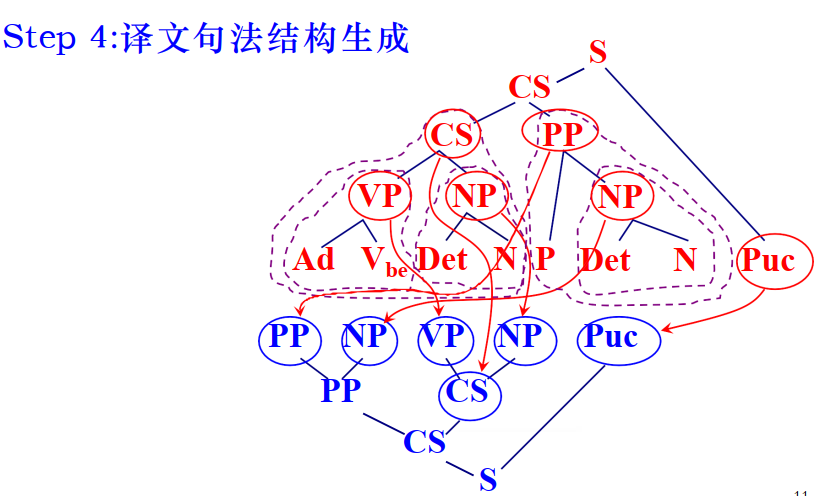
\includegraphics[width=0.6\linewidth]{fig/rule-based_mt.png}
\end{figure}

优点:保持原文结构、规范语句
\par 弱点:规则由人工编写,工作量大,主观性强,不利于系统扩充,灵活性低(对非规范语言现象无法处理)

\subsection{基于语料库的翻译方法}
\begin{figure}[H]
\centering
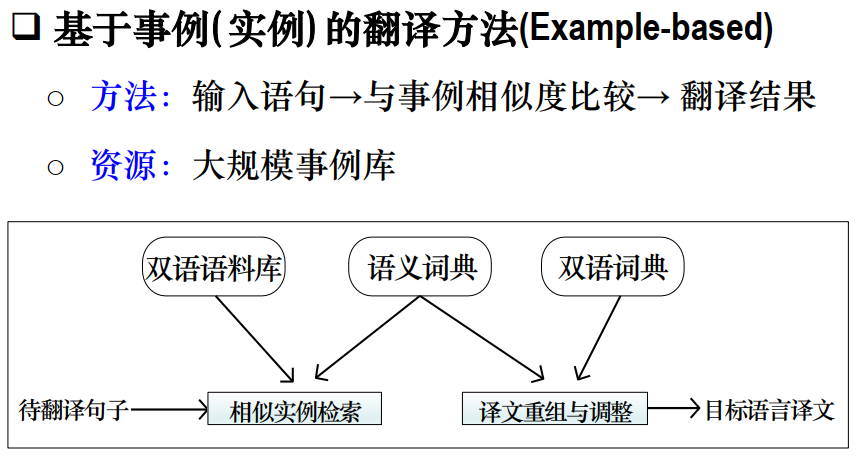
\includegraphics[width=0.6\linewidth]{fig/example-based_mt.png}
\end{figure}

\subsection{统计翻译}
\subsubsection{基本方法}
\begin{itemize}
	\item 源语言:$S=s_1^m=s_1s_2\cdots s_m$
	\item 目标语言:$T=t_1^l=t_1t_2\cdots t_n$
\end{itemize}
通过最大后验求解
\[\argmax_TP(T\mid S)=\argmax_T P(S\mid T)P(T)\]
其中$P(S\mid T)$为翻译模型(TM),确定了单词和词语如何被翻译(fidelity),从平行语料中学习;
$P(T)$为语言模型(LM),确定怎么写出好的目标语言的句子(fluency),从单语语料中学习。

三个关键问题:
\begin{itemize}
	\item 估计语言模型概率$P(T)$
	\item 估计翻译模型概率$P(S\mid T)$
	\item 快速搜索最大值解
\end{itemize}

\subsubsection{基于短语的翻译模型}
基于词的翻译模型很难消除歧义,很难处理一对多、多对一问题。
以短语为基本翻译单元,遵循短语划分、短语翻译、短语调序的步骤。
\begin{definition}[对齐一致性]
$S^j$中每个词$S_k$,若$(k,k')\in A$,则$i'\leq k'\leq j'$,$T_i^j$中每个词$T_{t'}$,若$(t,t')\in A$,则$i\leq t\leq j$。
\end{definition}

关键问题是学习短语翻译规则(双语句对词语对齐、短语翻译规则抽取)、估计短语翻译概率。

\subsection{神经机器翻译}
统计机器翻译都是人工设定的模块和特征,可解释性高、模块定制化、错误追踪,但是数据稀疏、不擅长复杂结构、依赖先验知识。

分布式的语义表示是统计机器翻译到机器翻译的核心
\begin{figure}[H]
\centering
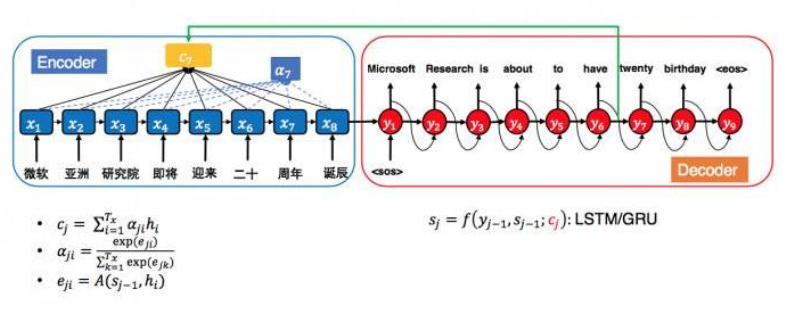
\includegraphics[width=0.6\linewidth]{fig/attention.png}
\end{figure}

BLEU(BiLingual Evaluation Understudy)评价方法:统计同时出现在系统译文和参考译文中的$n$元词个数,最后把匹配到$n$元词的数目除以系统译文的$n$元词数目,得到评测结果。